\subsection{Data Flow and Internal Logic}

The back-end of Uknow InfoHub system comprises mainly five components: item
fetcher, prefilter, data storage, postfilter and API website, as
illustrated in \figref{architecture}.
Data passing between modules are encoded using json formats.

\begin{figure}[H]
  \centering
  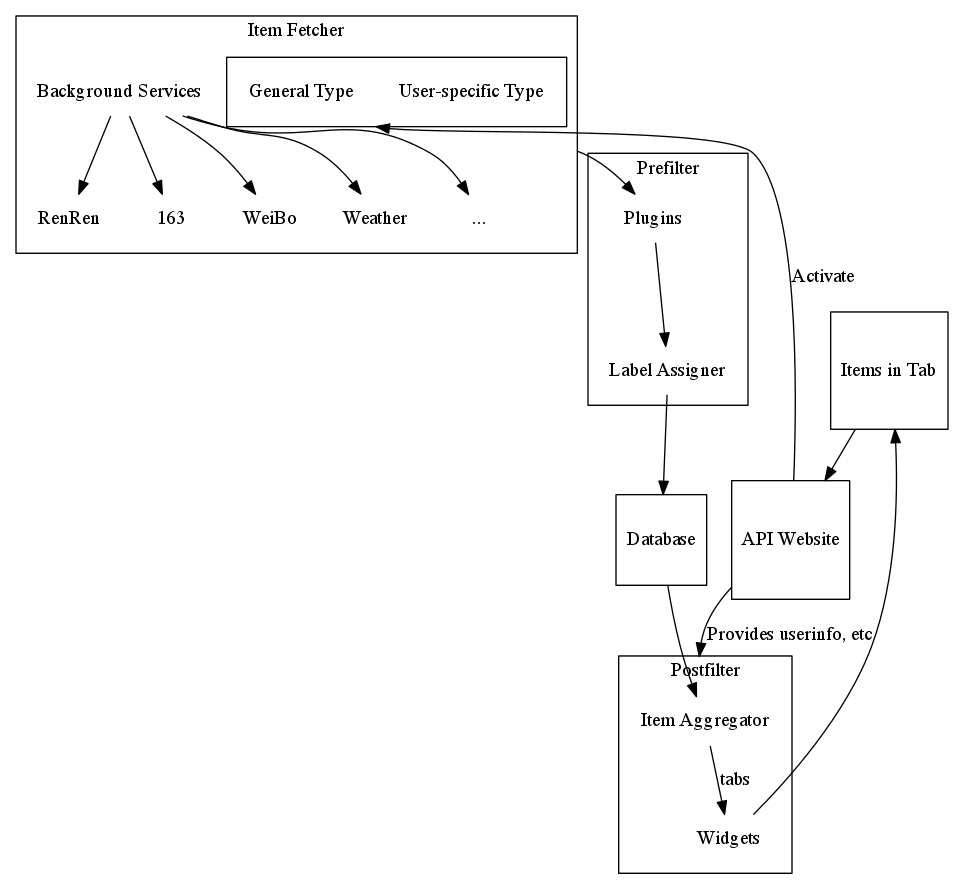
\includegraphics[width=\textwidth]{img/architecture.png}
  \caption{Overall architecture of Uknow backend\label{fig:architecture}}
\end{figure}


\subsubsection{Item}

An item is an abstract concept standing for a piece of collected
information to be presented to the user. It can be almost anything, such
as a status on SNS like renren, a piece of news from Netease, or a Weibo post
or tweets. An item is represented as a dictionary structure
programmatically. Following attributes are associated with an item:

\begin{enumerate}
\def\labelenumi{\arabic{enumi}.}
\itemsep1pt\parskip0pt\parsep0pt
\item
  An integer unique ID, which is used system-widely to identify a
  specific item.
\item
  Item fetcher type, which could be general item fetcher or aa
  user-specific item fetcher along with the user ID. See descriptions
  below for further details.
\item
  A set of labels, each of which describes a property of the underlying
  item. Possible labels include data source (websites such as renren,
  Facebook), data category (news, SNS updates, and etc.), and inferred
  information such as its importance to the user. An item could either
  be public or user-specific, and the associated labels could be
  different for different users.
\item
  A brief description as human-readable plain text, which could also be
  used for plugins involving NLP(nature language processing) and item
  searching.
\item
  Creation time
\item
  Other attributes for a specific item category.
\end{enumerate}

\subsubsection{Item fetcher}

\begin{figure}[H]
  \centering
  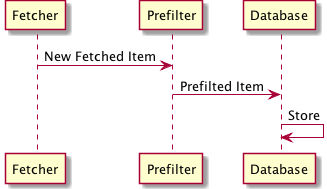
\includegraphics[width=0.6\textwidth]{img/fetch.png}
  \caption{Workflow of Fetcher \label{fig:fetcher}}
\end{figure}


Item fetchers simply retrieve items from various information sources,
adding basic attributes such as ID, description, source URL (if
available), and then forward items to prefilter for later processing, as illustrated in \figref{fetcher}.
There are two types of item fetcher:

\begin{description}
\item[General Item Fetcher]\hfill

  This kind of item fetcher collects public
 such as news and weather. They should always run in
  background and provide new data. No user login or authentication
  should be involved at this stage.
\item[User-specific Item Fetcher] \hfill

  This kind of item fetcher is activated by
  user action (such as login); when activated, it would collect
  information that could only be gained after authentication (such as
  connecting to SNS sites). The API website sends an activation signal
  along with corresponding user ID to all this kind of item fetchers,
  and they should do the work in background. Note that the activating
  process is asynchronous and the user could only get results of some
  time earlier to his request; however the latency should be fairly
  small if fast servers and Internet connection are guaranteed.
\end{description}

\subsubsection{Prefilter}

Prefilter is responsible for processing an item before putting it into
database. Prefilter consists of a series of plugins, each of which takes
the item dictionary as input and outputs a possibly modified item or
aborts processing of current item and discards it. This series comprises
two parts configured by the system administrator and the users
respectively. For the system-wide part, common plugins include infer
extra labels from item content or filtering illegal items. For items
produced by a user-specific item fetcher, plugins enabled by the
corresponding user is referred to as the ``user part'' and would be
applied on this item.

\subsubsection{Database Storage}

After processed by prefilter, if an item is not discarded, it would be
stored in the database. Due to the heterogeneous nature of data items,
we decided to use MongoDB as the storage back-end. The advantages would
be discussed later in \secref{data}.

\subsubsection{Postfilter}

Postfilter contains two stages:

\begin{enumerate}
\def\labelenumi{\arabic{enumi}.}
\itemsep1pt\parskip0pt\parsep0pt
\item
  Item Aggregator: When a user requests items in a tab, possibly with
  time, page number or seaching keyword constraints, the item aggratator
  simply finds items meeting those conditions and return them in some
  order.
\item
  Like prefilter, a sequence of system-wide and user-defined plugins are
  then applied to the items, which, for example, could deduplicate items
  in the same tab.
\end{enumerate}

\subsubsection{API Website}

\begin{figure}[H]
  \centering
  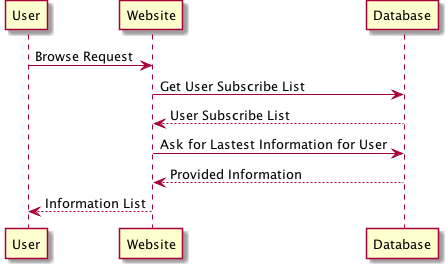
\includegraphics[width=0.6\textwidth]{img/browse.png}
  \caption{Workflow of the API website\label{fig:website}}
\end{figure}


API Website is the interface of the back-end system which interacts with
users, though indirectly. It accepts user requests, invokes
corresponding functions as described above, fetches and presents result
back to user, as displayed in \figref{website}. Refer to \secref{webapi} for further discussion about the API interfaces.

\subsection{Scalability}

\subsubsection{Data Storage}
\label{sec:data}
Data storage is implemented using MongoDB\footnote{\url{http://www.mongodb.org/}},
which is a leading NoSQL databse proven to be fast, stable, flexible and reliable.
Care has to be taken on creating
appropriate indexes to allow fast querying. Techniques such as
replication and sharding could be adopted to enhance efficiency and
reliability, only if there are enough servers. With the help of such
mature production, we do not have to worry too much about data storage.

\subsubsection{Background Workers}

As mentioned above, there are long running background workers fetching
items from public information sources. As the total number of such
sources is limited, it is not necessary to deploy many of those workers, and this
obviously has no scalability issue with growth of user group.

However, user-specific fetchers must be able to scale with the number of
users. Here we set up a worker cluster. The cluster contains a task
queue and distributed worker nodes. When a user activates a fetcher, a
task is added to the queue, and some worker node then picks up the task
and finishes it asynchronously. We choose
Celery\footnote{\url{http://www.celeryproject.org/}}, a distributed, asynchronous task queue to be the queue framework in Uknow.
For a worker node, it must be equipped with high-speed Internet
connection; and we can use co-routines (e.g., greenlet\footnote{\url{https://pypi.python.org/pypi/greenlet}} in Python)
to reduce CPU workload.

Now the system is fully horizontally scalable; theoretically a large
number of users could be served simultaneously if sufficiently many
servers are available.

\subsection{Availablity}

The key to increasing availability is to introduce redundancy. There
could be multiple queue schedulers and multiple worker nodes, failure of
any of which would not influence the whole system. The replication
mechanism provided by MongoDB also guaranteed the availability of data
storage. For API website, we could set up an Nginx\footnote{\url{http://wiki.nginx.org/Main}} server with reverse
proxy to multiple API servers, which makes the whole system almost as
reliable as anyone would request.

\subsection{Security}

The python drivers for MongoDB makes it impossible to commit attacks like SQL
injection. It is hard for our system itself to contain any security
vulnerabilities. Care has to be taken on system security such as server
software, operating system configuration and etc.
